\documentclass[letterpaper]{article}
\DeclareSymbolFont{AMSb}{U}{msb}{m}{n}
\DeclareMathAlphabet{\mathbbm}{U}{bbm}{m}{n}

\title{Ends}

\usepackage{amsmath,amssymb,amsthm,latexsym}
\usepackage[cm]{fullpage}
\usepackage{bm}
\usepackage{tikz}
 \usetikzlibrary{arrows,calc,matrix,positioning,scopes}
\usepackage{textcomp}
\usepackage{mathtools}
\usepackage{hyperref}
% http://tex.stackexchange.com/questions/52410/how-to-use-the-command-autoref-to-implement-the-same-effect-when-use-the-comman
\def\equationautorefname~#1\null{(#1)\null}

\DeclarePairedDelimiterX\angles[1]{\langle}{\rangle}{#1}
\DeclarePairedDelimiterX\angbar[1]{\langlebar}{\ranglebar}{#1}
\DeclarePairedDelimiterX\paren[1]{(}{)}{#1}
\DeclarePairedDelimiterX\brak[1]{[}{]}{#1}
\DeclarePairedDelimiterX\abs[1]{\lvert}{\rvert}{#1}
\DeclarePairedDelimiterX\set[1]{\{}{\}}{#1}

% http://tex.stackexchange.com/questions/5502/how-to-get-a-mid-binary-relation-that-grows
\DeclareMathOperator{\mmid}{\mathrel{}\mathclose{}\delimsize|\mathopen{}\mathrel{}}

\newcommand{\defn}[1]{{\bf #1}}
\newcommand{\Hom}[3]{\textrm{Hom}_{#1}{\paren{#2,#3}}}

\renewcommand{\baselinestretch}{0.9}

\begin{document}

Readers of this document should perhaps have first made an effort to read
Bartosz Milewski's \textit{Natural Transformations and Ends} (at
\url{http://bartoszmilewski.com/2014/07/15/natural-transformations-and-ends/}).
This document emerged from my attempting to understand that one; it covers
the same topic with a different presentation order.

\section{Introduction, or, Ends: A Means to What End?}

Consider a strongly-typed, functional programming language.  Traditionally,
we embed the semantics of such things into category theory by constructing a
category where the objects are {\em types} of the language and morphisms are
{\em constructable functions}: the composition closure of primitives and
expressible $\lambda$ terms.  The category must be Cartesian-closed, if we
want to embed functions, because we need exponential objects: they
correspond to $\to$-typed objects.

In fact, there's a natural tool that goes a great distance in helping us
here.  The $\text{Hom}_{\mathbf{C}}$ diagonal bifunctor.  Given any two
objects in $\mathbf{C}$, it gives us the {\em set} of arrows between them.

A glaring deficiency of this embedding, however, is the complete lack of
polymorphism.  There is no one ``identity function'' in this story, rather,
there is one at every type.  We can work around this by viewing prenex
polymorphism (that is, all universal quantifiers scope over the entire type)
as a {\em metatheoretic} instrument.  We can adjust our proof rules which
map a program to its categorical form to, essentially, defer computation of
which categorical object or morphism is in play until {\em after} enough
type information is available.  Such treatments typically render the
polymorphic identity function as $(\Lambda_{\alpha : \star} \lambda_{x :
\alpha} x) : \forall_{\alpha : \star} . \alpha \to \alpha$, for example,
making explicit the type-level binder.  Hand waving a bit, the (usually
STLC) program whose terms are terms of the language, $\Lambda$-bound
functions, and (type) applications is then evaluated to obtain the
underlying monomorphic program, which can then be given categorical
semantics.

But that clever trick breaks down if we have non-prenex polymorphism, where
we can actually give a binder whose type involves a universal quantifier.
Such an expression might be $(\Lambda_{\alpha : \star} \lambda_{f :
\Lambda_{\beta : \star} . \beta \to \beta} \lambda_{x . \alpha} f~\alpha~x)
: \forall_{\alpha : \star} (\forall_{\beta : \star} . \beta \to \beta) \to
\alpha \to \alpha$.  (This is not intended to be a terribly {\em useful}
example, just illustrative.)  Here we see that we have a type variable
$\alpha$ quantified in prenex position, and another, $\beta$, whose
quantifier cannot be moved higher.  Put a different way, $f$ is drawn from
{\em the set of polymorphic functions} $\forall_{\alpha : \star} . \alpha
\to \alpha$.  If we want to give categorical semantics to this object, we
need an object that represents that set.%
%
\footnote{I believe this intuition describes an {\em impredicative} system,
like System F, since $\star$ includes the object representing
$\forall_{\alpha : \star} . \alpha \to \alpha$.}

If we think about it, though, we see that a particular term $\Lambda_{\alpha
: \star} \phi(\alpha) : \forall_{\alpha : \star} \tau(\alpha)$ is really a
$\alpha$-indexed {\em product} (For each $a \in \alpha$, there is a
$\phi(a)$.)  Of course, there may be multiple $\phi(\alpha)$ terms that all
have the type $\tau(\alpha)$, so the collection of all terms of type
$\forall_{\alpha : \star} \tau(\alpha)$ is a {\em two-indexed collection} of
terms.  This is the end!

\section{Natural Transformations As Parametric Polymorphism}

Any parametrically-polymorphic function, let's call it $\eta$, will have a
type with a $\forall_{\tau : \star}$ quantifier scoping over a $\to$
constructor whose the two arguments are type-level functions of $\tau$.
That is, it will have type $\forall_{\tau : \star} F \tau \to G \tau$, for
some type-level functions $F$ and $G$.

%at the term level, we know that the $\eta$-long%
%%
%\footnote{Apologies; there are only so many Greek letters and the standard
%usages clash.}
%%
%form of $\eta$ is $\Lambda_{\tau : \star} \lambda_{x : F \tau} (\phi~\tau~x
%: G \tau)$ for some $\phi$.

In order for us to justify the term ``parametric'', it should be the case
that two instantiations of such a function, say, at types $\tau$ and
$\tau'$, ``behave similarly''.  We can give an exact meaning to this when
$F$ and $G$ are in fact {\em functors}, not just type-level functions: if
there is some function $f : \tau \to \tau'$, then these two paths of getting
from $F \tau$ to $G \tau'$ must be equal if we are to say that $\eta~\tau$
and $\eta~\tau'$ ``behave similarly''; this is just the {\em definition} of
a natural transformation $\eta : F \stackrel{\cdot}{\to} G$:

\begin{center}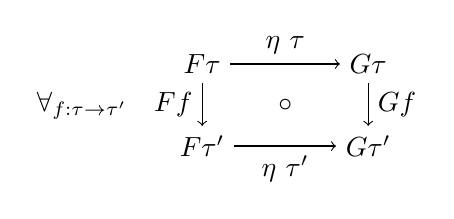
\begin{tikzpicture}
%
  \matrix[matrix of math nodes,column sep={60pt,between origins},
          row sep={30pt,between origins}] (m) {
%
  |[name=mtl]| F \tau  & |[name=mtr]| G \tau \\
  |[name=mbl]| F \tau' & |[name=mbr]| G \tau' \\
%
  } ;
%
  \node at ($(m.west)+(-1,0)$) {$\forall_{f : \tau \to \tau'}$} ;
  \draw [->] (mtl) -- (mtr) node [above,midway] {$\eta~\tau$} ;
  \draw [->] (mbl) -- (mbr) node [below,midway] {$\eta~\tau'$} ;
  \draw [->] (mtl) -- (mbl) node [left ,midway] {$F f$} ;
  \draw [->] (mtr) -- (mbr) node [right,midway] {$G f$} ;

  \node at (m) {$\circ$};
\end{tikzpicture}\end{center}

The diagram is essentially unchanged if $F$ and $G$ are {\em contravariant}
functors instead.  I do not know how to formalize ``parametric'' when $F$
and $G$ are not functors (of either variance).

\section{Profunctors}

A profunctor is a bifunctor (it may be helpful to review
\url{bifunctors.pdf}) with one argument of each variance (typically, and
here, the first is the contravariant one).  That is, a profunctor $S :
\mathbf{A}^{\text{op}} \times \mathbf{B} \to \mathbf{C}$ has two maps:
$S~A~B$, mapping pairs of objects to objects; and $S~f~g : S~A'~B \to
S~A~B'$ mapping pairs of arrows to arrows, where $A,A' \in \mathbf{A}_0$,
$B,B' \in \mathbf{B}_0$, $f : A \to A' \in \mathbf{A}_1$, and $g : B \to B'
\in \mathbf{B}_1$.  We know that the arrow map preserves identity and
composition, though we will not actually need these facts.%
%
\footnote{For the curious, however, that is: $S~id_A~id_B = id_{S A B}$ and
given, additionally, $f' : A' \to A'' \in \mathbf{A}_1$ and $g' : B' \to B''
\in \mathbf{B}_1$, then $S~(f \circ f')~(g \circ g') : S~A''~B \to S~A~B''$
is the composition of $S~f~g' : S~A'~B' \to S~A~B''$ and $S~f'~g : S~A''~B
\to S~A'~B'$.}

When $\mathbf{A} = \mathbf{B}$, we may call $S$ a ``diagonal profunctor''.
Such a thing generalizes $\text{Hom}$ by producing ``$\text{Hom}$-like
constructs'' in its target category and capturing both pre- and
post-composition.  The objects in the image of a profunctor are objects that
can play the role of bundles of arrows of the source category.

\section{A Particular Diagonal Profunctor}
\label{sec:apdp}

Recall, the ultimate goal is to find a categorical object (in
$\mathbf{Set}$) that captures the set of natural transformations between two
functors $F$ and $G$.  The two paths through a natural transformation
diagram for $\eta : F \stackrel{\cdot}{\to} G$ and $f : \tau \to \tau'$ are
$(\eta~\tau') \circ (F f)$ and $(G f) \circ (\eta~\tau)$.  Someone with a
great deal more insight than this author realized that these are images of a
particular diagonal profunctor $S_{\text{nat},F,G}$ defined on objects by
$S_{\text{nat},F,G}~\tau~\tau' = \text{Hom}~\tau~\tau'$ and on arrows by
%
\[ (S_{\text{nat},F,G}~(f : \tau \to \tau')~(g : \tau'' \to \tau'''))~(h :
\text{Hom}~\tau'~\tau'') = (G g) \circ h \circ (F f) :
\text{Hom}~\tau~\tau'''.\]
%
In particular, our two paths appear in the {\em off-diagonal}
$S_{\text{nat},F,G}~\tau~\tau'$ as the $S_{\text{nat},F,G}~f~id_{\tau'}$
image of $\eta~\tau'$ (in $\text{Hom}~\tau'~\tau'$) and the
$S_{\text{nat},F,G}~id_{\tau}~g$ image of $\eta~\tau$ (in
$\text{Hom}~\tau~\tau$).  Recall, the definition of a natural transformation
says that these two images must be equal; the question facing us now, then,
is how to encode this fact categorically.

Some object $N$ can be used to index the collection of natural
transformations between $F$ and $G$ if it comes equipped with projectors
$\pi~\alpha$ for every $\alpha : \star$ such that $\pi~\alpha~\eta$ (for
each $\eta \in N$) is the $\alpha$-th component of $\eta$.

Drawing the conclusions of the above two paragraphs at once, we have this
rendering of our seemingly so simple equation $G f \circ (\eta~\tau) =
(\eta~\tau') \circ F f$ (admittedly, for all natural transformations
$\eta$):
%
\begin{center}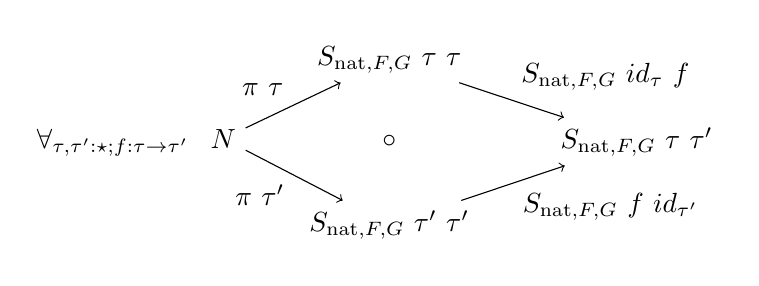
\begin{tikzpicture}
%
  \matrix[matrix of math nodes,column sep={60pt,between origins},
          row sep={30pt,between origins}] (m) {
%
  & |[name=t]| S_{\text{nat},F,G}~\tau~\tau \\
  |[name=l]| N & & |[name=r]| S_{\text{nat},F,G}~\tau~\tau' \\ 
  & |[name=b]| S_{\text{nat},F,G}~\tau'~\tau' \\
%
  } ;
%
  \node at ($(m.west)+(-1,0)$) {$\forall_{\tau,\tau' : \star; f : \tau \to \tau'}$} ;
  \draw [->] (l) -- (t) node [above left,midway] {$\pi~\tau$} ;
  \draw [->] (l) -- (b) node [below left,midway] {$\pi~\tau'$} ;
  \draw [->] (t) -- (r) node [above right,midway] {$S_{\text{nat},F,G}~id_{\tau}~f$} ;
  \draw [->] (b) -- (r) node [below right,midway] {$S_{\text{nat},F,G}~f~id_{\tau'}$} ;
  \path (t) -- (b) node [midway] {$\circ$} ;

\end{tikzpicture}\end{center}

We could imagine that there are many such $N$ (and their associated $\pi$
projector bundles) that made the above diagram work.  If, however, there is
a {\em universal} one, $E$, such that:
%
\begin{center}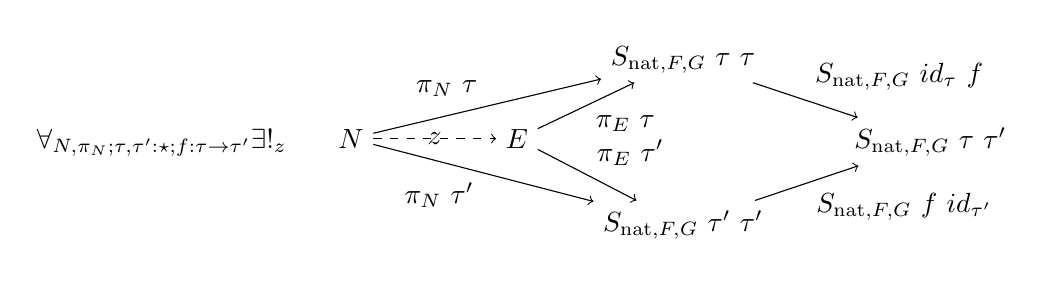
\begin{tikzpicture}
%
  \matrix[matrix of math nodes,column sep={60pt,between origins},
          row sep={30pt,between origins}] (m) {
%
  & & |[name=t]| S_{\text{nat},F,G}~\tau~\tau \\
  |[name=l]| N & |[name=e]| E & & |[name=r]| S_{\text{nat},F,G}~\tau~\tau' \\ 
  & & |[name=b]| S_{\text{nat},F,G}~\tau'~\tau' \\
%
  } ;
%
  \node at ($(m.west)+(-2,0)$) {$\forall_{N, \pi_N; \tau,\tau' : \star; f : \tau \to
  \tau'}\exists!_{z}$} ;
  \draw [dashed,->] (l) -- (e) node [midway] {$z$} ;
  \draw [->] (l) -- (t) node [above left,midway] {$\pi_N~\tau$} ;
  \draw [->] (l) -- (b) node [below left,midway] {$\pi_N~\tau'$} ;
  \draw [->] (e) -- (t) node [below right,midway] {$\pi_E~\tau$} ;
  \draw [->] (e) -- (b) node [above right,midway] {$\pi_E~\tau'$} ;
  \draw [->] (t) -- (r) node [above right,midway] {$S_{\text{nat},F,G}~id_{\tau}~f$} ;
  \draw [->] (b) -- (r) node [below right,midway] {$S_{\text{nat},F,G}~f~id_{\tau'}$} ;

\end{tikzpicture}\end{center}
%
Then this $E = \text{End}(S) = \int S = \int_\tau S~\tau~\tau$ is the
\textbf{end} of the profunctor $S_{\text{nat},F,G}$.  It represents the
collection of all $F \stackrel{\cdot}{\to} G$.%
%
\footnote{The use of the $\int$ symbol is unfortunate, but standard; as
discussed above, the end is much more like a product than a sum.  Note the
direction of the arrows in its definition diagram and compare to the
universal diagram defining a product!}

\section{Generalizing: Dinatural Transformations and Generalized Limits}

We can generalize the notion of a natural transformation between two
functors to a ``dinatural transformation'' (for ``diagonally-natural'')
between two diagonal profunctors.  Like a natural transformation, a
dinatural transformation is a quiver of arrows; possibly surprisingly, the
quiver will continue to be a single-indexed object on objects of
$\mathbf{A}$.  Concretely, $\theta : R \stackrel{\bullet}{\to} S$ is a
dinatural transformation if
%
\begin{center}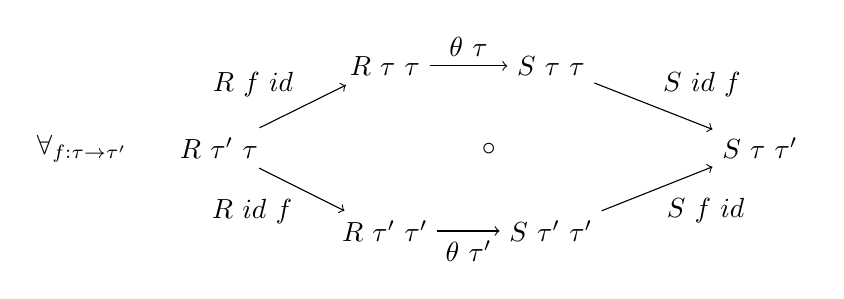
\begin{tikzpicture}

  \matrix[matrix of math nodes,column sep={60pt,between origins},
          row sep={30pt,between origins}] (m) {
%
  & |[name=mtl]| R~\tau~\tau & |[name=mtr]| S~\tau~\tau \\
  |[name=l]| R~\tau'~\tau    & & & |[name=r]| S~\tau~\tau' \\
  & |[name=mbl]| R~\tau'~\tau'   & |[name=mbr]| S~\tau'~\tau' \\
%
  } ;

  \node at (m) {$\circ$} ;
  \node at ($(m.west)+(-1,0)$) {$\forall_{f : \tau \to \tau'}$} ;

  \draw [->] (l) -- (mtl) node [above left,midway] {$R~f~id$} ;
  \draw [->] (l) -- (mbl) node [below left,midway] {$R~id~f$} ;

  \draw [->] (mtl) -- (mtr) node [above,midway] {$\theta~\tau$} ;
  \draw [->] (mbl) -- (mbr) node [below,midway] {$\theta~\tau'$} ;

  \draw [->] (mtr) -- (r) node [above right,midway] {$S~id~f$} ;
  \draw [->] (mbr) -- (r) node [below right,midway] {$S~f~id$} ;

\end{tikzpicture}\end{center}

If we define a ``constant bifunctor'' $\kappa~\tau~\tau' = N$ and
$\kappa~f~g = id_N$, then our $S_{\text{nat},F,G}$-based rendering of
natural transformations' equation in \autoref{sec:apdp} above is a dinatural
transformation $\kappa \stackrel{\bullet}{\to} S_{\text{nat},F,G}$!

Recall that a limit of a diagram $\mathbf{J}$ included into $\mathbf{C}$ by
a full and faithful functor $F$ is the terminal object in the subcategory of
$C$ whose objects $C_\kappa$ are selected by constant functors $\kappa :
\mathbf{J} \to \mathbf{C}$ with natural transformations $\eta_\kappa :
\kappa \stackrel{\cdot}{\to} F$ and whose arrows $z : C_\kappa \to
C_\kappa'$ indicate factoring of $\eta_\kappa~\tau = \eta_{\kappa'}~\tau
\circ z$.  (Phew!)

We can generalize this notion to use {\em dinatural transformations}.  Given
an indexing category $\mathbf{J}$, and a diagonal profunctor $S :
\mathbf{J}^{\text{op}} \times \mathbf{J} \to \mathbf{C}$ we're now
interested in the subcategory of objects $C_\kappa$ picked out by constant,
diagonal profunctors $\kappa$ (of the same type as $S$) which have dinatural
transformations to $S$ ($\kappa \stackrel{\bullet}{\to} S$).  The terminal
object in this subcategory, if there is one, is the end of $S$.

\section{Preliminary Thoughts: Parametricity Without Functors}

Above, we restricted our attention to the case where the type constructors
$F$ and $G$ were in fact functors.  We made heavy use of this fact in
defining $S_{\text{nat},F,G}$, whose End we then characterized.

We can view the natural transformation diagram as simply the assertion that
$\forall_{\tau,\tau' : \star; f : \tau \to \tau'} \exists!_{\eta_f : F \tau
\to G \tau'} .  \eta_f = \eta~\tau' \circ F f = G f \circ \eta~\tau$, or,
equivalently, that for each $\eta : F \stackrel{\cdot}{\to} G$ there is a
function, which we might also call $\eta$, of type $\forall_{\tau,\tau' :
\star} (\tau \to \tau') \to (F \tau \to G \tau')$ such that $\eta~f =
\eta~\tau' \circ F f = G f \circ \eta~\tau$.%
%
\footnote{I am indebted to ``ski'' of \texttt{\#haskell} on Freenode for a
reminder of this view and the name $\eta_f$.}
%
We could in fact take {\em this} $\eta$ as the definition of a parametric
function: rather than being a type-indexed collection of functions, a
parametric function is then a type-indexed collection of {\em higher-order}
functions.  When $F$ and $G$ are functors, we can use either to implement
and adaptor function of the right type: $\lambda_{\eta : \forall_{\beta :
\star} F \beta \to G \beta} \Lambda_{\alpha,\alpha':\star} \lambda_{f :
\alpha \to \alpha'} \lambda_{x : F \alpha} (G~f)~(\eta~\alpha~x)$ or
$\eta~\alpha'~((F~f)~x)$ under identical binders.

If only $F$ is a functor, we could still impose an equation of the form
$\eta~(f : \tau \to \tau')~(x : F \tau) = \eta~id_{\tau'}~((F~f)~x)$ (at $G
\tau'$).  That is, the function $\eta$ cannot distinguish between being
given a function $f$ and some data $x$ and being given the identity function
and the data $(F~f)~x$. 

\end{document}
